\section{Work Breakdown Structure}

A Work Breakdown Structure is a method to visualize the workflow of the project. In the figure below, a full breakdown of the project is shown.

\begin{figure}[H]
    \centering
    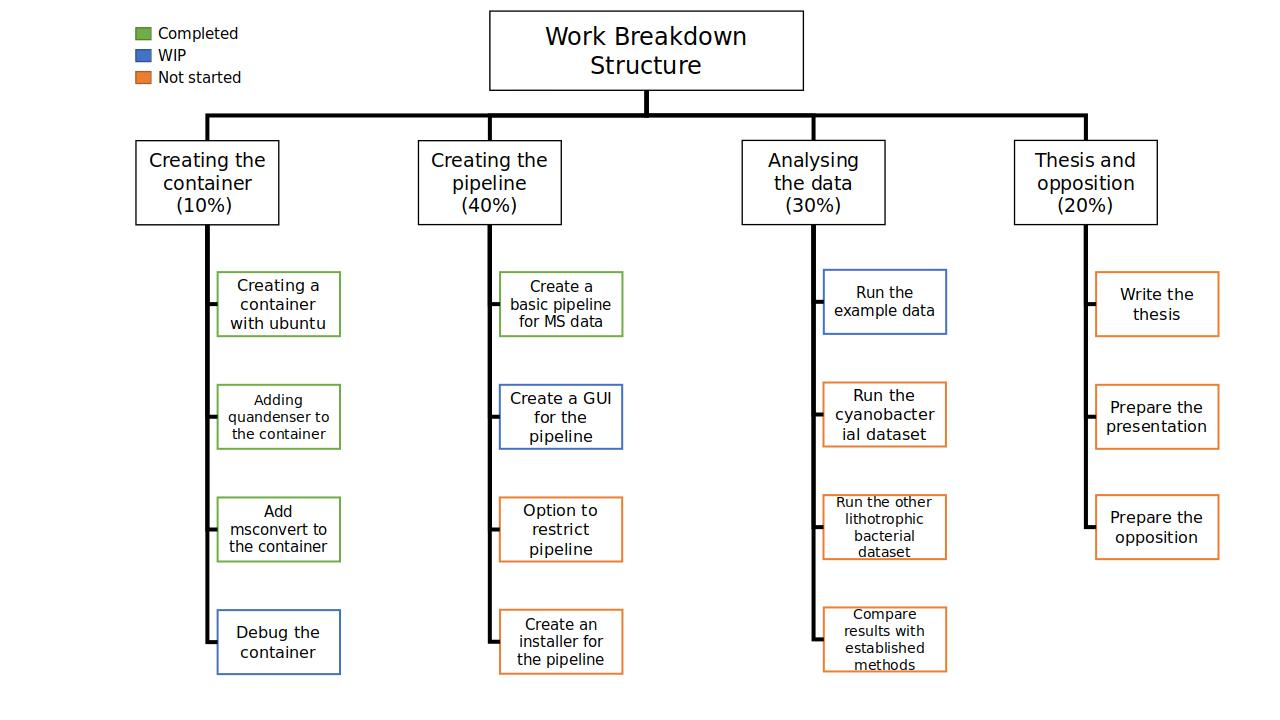
\includegraphics[width=\textwidth,height=\textheight,keepaspectratio]{Pictures/wbs.jpg}
    \caption{Work Breakdown Structure of the project. The percentages are the allocated time for each part of the project. The colors indicate which parts have been completed, are currently worked on or have not been started yet}
\end{figure}
